\documentclass[compress]{beamer} %en animé
%\documentclass[trans]{beamer} %en superposé

\usepackage{graphicx}
\usepackage{tabularx}
\usepackage{listings}


%%%%%%%%%%%%%% LES PACKAGES
%-------------------
\usepackage[utf8]{inputenc}
\usepackage[T1]{fontenc}
\usepackage[frenchb]{babel}
%\usepackage[english]{babel}

%-------------------
\usepackage{minted} %pour inclure du code
\setminted[ocaml]{	                               
	%bgcolor = black!3!white,                           %--fond 
	frame = leftline,	framesep = 6pt, rulecolor= expli, %-- cadre
	linenos=true, numbersep=4pt, xleftmargin=20pt,      %--numéro de ligne
	breaklines=true,                                    %--découpage des longues lignes
	tabsize=2,                                          %--tabulations
}
\setminted[c]{	                               
	%bgcolor = black!3!white,                           %--fond 
	frame = leftline,	framesep = 6pt, rulecolor= expli, %-- cadre
	linenos=true, numbersep=4pt, xleftmargin=20pt,      %--numéro de ligne
	breaklines=true,                                    %--découpage des longues lignes
	tabsize=2,                                          %--tabulations
}

%-------------------
\usepackage[ruled,vlined]{algorithm2e} %pour le pseudo-code
%ajouter l'option linesnumbered si on veut les numéros de lignes
\SetAlgorithmName{Algorithme}{Algo}{Liste des algorithmes}
\SetFuncArgSty{textup}%style des arguments des fonctions pas en gras
\SetArgSty{textup}%style des condidtions des if, for, while pas en gras


\SetKwFor{ForEach}{pour tout}{faire}{}
\SetKwFor{For}{pour}{faire}{finpour}
\SetKwIF{Si}{SinonSi}{Sinon}{si}{alors}{sinon si}{sinon}{}
\SetKwInput{Input}{Entrée}
\SetKwInput{Output}{Sortie}
\SetKwProg{myproc}{Procedure}{:}{}
\SetKw{Return}{retourner}
\SetKwComment{tcc}{(*}{*)}
\SetKwFor{Tq}{tant que}{faire}{}
\SetKwRepeat{Repeter}{répéter}{jusqu’à}

%-------------------
\usepackage{amsmath,amsfonts,amssymb}
\usepackage{textcomp,lmodern}%pour l'euro
\usepackage{cancel}%pour barrer

%-------------------
\usepackage{array,multirow}
\usepackage{tabularx}%tableaux élastiques


%-------------------
\usepackage{tikz} %graphiques et dessins
\usetikzlibrary{shapes}%pr écrire \node[ellipse] par ex
\usetikzlibrary{positioning} %pr écrire \node[below rigth = 3pt and 5pt]
\usetikzlibrary{decorations.pathreplacing}%pr les accolades
\usetikzlibrary{patterns}%pour les hachures

%-------------------
\usepackage{caption}%les personaliser (les centrer par ex)
\usepackage{changepage}%pour élargir la page avec adjustwidth
\usepackage{calc}%pour pouvoir écrire \textwidth-1cm


%-------------------
\usepackage{xspace}%espaces après les commandes texte


%------------------

%-------------------



\usepackage[clock]{ifsym}

%%%%%%%%%%%%%% THEME BEAMER
%votre nom court qui apparaîtra dans l'en tête
\newcommand{\initiales}{Burgalat.E }
\usetheme{Montpellier}
\usecolortheme{seahorse}

%--------marges
\setbeamersize{text margin left= 0.7cm}
\setbeamersize{text margin right= 0.7cm}

%--------tête et pieds
\setbeamertemplate{navigation symbols}{}
\setbeamertemplate{footline}[frame number]
\setbeamertemplate{headline}{
  %la premiere ligne
  	\begin{beamercolorbox}[ht=0.42cm, vmode]{section in head/foot}
	\hspace{0.4cm} \insertshorttitle 
	\hspace*{0.1cm}- \initiales - {\insertshortdate}
	\vspace*{0.08cm} 
  	\end{beamercolorbox}
  %la deuxième ligne
	\begin{beamercolorbox}[ht=0.4cm, vmode]{subsection in head/foot}
	%titre de la section si elle est pas 0
		\ifnum\value{section}=0{} 
		\else{ \hspace{0.8cm} \thesection - \insertsectionhead }
		\fi
	%séparateur + titre de la sous-section si elle est pas 0
		\ifnum\value{subsection}=0{} 
		\else{ 
			\hspace*{0.1cm} \couleur{$\bullet$} \hspace*{0.1cm} 
			\thesection.\thesubsection \, \insertsubsectionhead
		}
		\fi
		\vspace*{0.12cm}
\end{beamercolorbox}
%\vspace*{-0.03cm} %pour pas qu'il y ait d'espace avec la ligne de frametitle
 }
%\setbeamertemplate{frametitleheigth}{4cm}
\setbeamertemplate{frametitle}{
	\vspace*{-0.04cm} 
	\begin{beamercolorbox}[ht=0.8cm,wd=\paperwidth, vmode]{frametitle}
		\hspace{0.3cm} \insertframetitle \vspace*{0.1cm}
	\end{beamercolorbox}
}

%commande pour ajuster l'alignement vertical des titres sans lettres descendantes
%\newcommand{\esp}{\\[0.1cm]} %--version qui marche sans le package minted
\newcommand{\esp}{\\[-0.5cm]} %--version qui marche avec le package minted


%--------couleurs
\setbeamercolor{structure}{fg=prunelle!70!black} 

\setbeamercolor{block title}{fg=turquoiseFonce!70!black,bg=vertdEau}
\setbeamercolor{block body}{bg=vertdEau!10!white}

\setbeamercolor{block title alerted}{bg=vertdEau!85!white,fg=turquoiseFonce!80!black}
\setbeamercolor{block body alerted}{bg=vertdEau!8!white}
%\setbeamercolor{alerted text}{fg=red}

\setbeamercolor{block title example}{bg=vertdEau,fg=turquoiseFonce}
\setbeamercolor{block body example}{bg=vertdEau!10!white}
\setbeamercolor{example text}{fg=blue!20!turquoise}

%-------- TOC
\setbeamertemplate{section in toc}[sections numbered]

%-----------------------------------------------
%Plan qui s'affiche au début de chaque section %|
\AtBeginSection[]{                             %|
\begin{frame}[plain]                           %|
\frametitle{Plan\\[0.1cm]}                     %|
\tableofcontents[                              %|
currentsection,                                %|
hideothersubsections,                          %|
subsubsectionstyle=hide]                       %|
\addtocounter{framenumber}{-1}                 %|
\end{frame}}                                   %|
%-----------------------------------------------




%-------- commande pour les ref sur les slides
\newcommand{\bandeauREF}[1]{
\noindent\makebox[\textwidth][l]{%
\hspace{-\dimexpr\oddsidemargin+1in}%
\colorbox{expli!20!white}{%
\parbox{\dimexpr\paperwidth-2\fboxsep}{
\footnotesize\textcolor{expli!80!black}{#1}
}}}}



%%%%%%%%%%%%%% MA PALETTE DE COULEURS
%%%%%%%%%%%%%% couleurs locales
\newcommand{\cearly}{orange!50!oranger}
\newcommand{\ctardy}{orange!50!oranger!50!magenta!50!violet}
\newcommand{\cmilieu}{yellow!45!magenta}
\newcommand{\cfenetre}{yellow!45!magenta}
%\newcommand{\cfenetre}{orange!80!magenta!80!violet}
\newcommand{\caxe}{blue!60!black}

\definecolor{vert}{RGB}{194, 247, 50}
\definecolor{vertClair}{RGB}{80, 180, 33}
\definecolor{vertFonce}{RGB}{20, 148, 20} 


\definecolor{turquoiseFonce}{RGB}{0, 149, 182} 
\definecolor{turquoise}{RGB}{0, 204, 203}
%\definecolor{turquoise}{RGB}{53, 123, 153} 
\colorlet{monCyan}{turquoise!90!blue} 

\colorlet{vertdEau}{blue!50!green!30!white} 

\definecolor{prec}{RGB}{128, 0, 128} 
\definecolor{hyp}{RGB}{255, 0, 127} 


\definecolor{orange}{RGB}{250, 130, 1}
\definecolor{orange1}{RGB}{244, 142, 3}
\definecolor{orange2}{RGB}{255, 195, 0}
%\colorlet{orangé}{orange!55!yellow}
\colorlet{oranger}{orange!55!yellow}
\definecolor{jaune}{RGB}{255, 195, 0 }
\colorlet{ocre}{orange!90!green!80!white} 


\definecolor{briqueRouge}{RGB}{200, 48, 24}
\definecolor{brique}{RGB}{141, 48, 24}
\definecolor{brown}{RGB}{165, 137, 107}
\definecolor{chamois}{RGB}{200, 141, 75}

\colorlet{lavande}{vertdEau!50!blue}
\definecolor{lilas}{RGB}{154, 107, 165}
\colorlet{parme}{magenta} %violet!30!magenta
\definecolor{mauve}{RGB}{161, 132, 220}%{147, 112, 219}

\definecolor{prunelle}{RGB}{106,24, 141}
\definecolor{prune}{RGB}{121, 7, 123}
\definecolor{violet}{RGB}{153, 0, 139}
\definecolor{violette}{RGB}{128, 0, 128} 

\definecolor{rose}{RGB}{255, 0, 127} 
\definecolor{framboise}{RGB}{141, 24, 59}
\colorlet{grenat}{magenta!90!red!80!black}

\colorlet{expli}{gray}

\definecolor{hellseahorse}{RGB}{204, 204, 255}
\definecolor{seahorse}{RGB}{204,180, 255}
\definecolor{darkseahorse}{RGB}{83, 74, 196}

%symboles pratiques
\newcommand{\flch}{\item[$\rightarrow$]}
\newcommand{\dc}{{\usebeamercolor[fg]{structure}$\hookrightarrow$}}
\newcommand{\ok}{\textcolor{vert}{\checkmark}}
\newcommand{\point}{{\usebeamercolor[fg]{structure}$\bullet\enskip$}}
\newcommand{\Point}{{\usebeamercolor[fg]{structure}$\bullet\enskip$}}


%styles
\newcommand{\couleur}[1]{{\usebeamercolor[fg]{structure}#1}}
\newcommand{\important}[1]{\couleur{\textbf{#1}}}
\newcommand{\remarque}[1]{\textit{\textrm{#1}}}

%pour le template
\newcommand{\lin}[1]{\mintinline{latex}{#1}}
%%%%%%%%%%%%%%%%%%%%%%%%%%%%%%%%%%%%%%%%%%%%%%%%%
\begin{document}
%

%%%%%%%%%%%%%%%%%%%%%%%%%%%%%%%%%%%%%%%%%%%%%%%%%
% A COMPLETER 
%%%%%%%%%%%%%%%%%%%%%%%%%%%%%%%%%%%%%%%%%%%%%%%%%

%entre crochet le titre court pour l'en tête puis le vrai titre
\title[Gros titre : et sous titre (version courte)]{
Le Ray Marching :\\
{\large avec éventuellement un sous titre }
}

\author{
\large 
Présentation de \important{Eliot Burgalat}\\[0.2cm]
\footnotesize
travail réalisé avec \couleur{Tom Garcia}\\[0.4cm]
\vspace*{-1.2cm}
} 

%entre crochet la short date pour l'en-tête
\date[Juillet 2024]{}

\institute{}


%------------------------------------------------
\begin{frame}[plain]
\titlepage 
\addtocounter{framenumber}{-1} 
\end{frame}

%------------------------------------------------
\title[Ray marching : et sous titre (version courte)]{
Une page de titre avec logos :\\
{\large mais sans les affectations détaillées des auteurs }
}

%------------------------------------------------


%%%%%%%%%%%%%%%%%%%%%%%%%%%%%%%%%%%%%%%%%%%%%%%%%
\section[Première section]{Introduction}

%++++++++++++++++++++++++++++++++++++++++++++++++
\subsection{Principe de Ray Marching}


%------------------------------------------------
\begin{frame}
\frametitle{Ce qui apparaît dans l'en-tête}

Dans la \important{première ligne}:
\begin{itemize}
\flch la version courte du titre, précisée en option  de  \texttt{$\backslash$title}\\
\remarque{( en option = entre crochets, avant les accolades)}
\flch la version courte du nom, voire des initiales, redéfinir la commande
\texttt{$\backslash$newcommand\{$\backslash$initiales\}\{Petit Nom \}} 
\flch la version courte de la date, précisée en option de \texttt{$\backslash$date}\\
\end{itemize}
\bigskip
Dans la \important{deuxième ligne}:
\begin{itemize}
\flch le numéro et le titre de la section, sauf si le numéro est nul\\
\remarque{s'il est précisé en option de} \texttt{$\backslash$section}
\remarque{le titre court est utilisé}
\flch le numéro et le titre de la sous-section, sauf si le numéro est nul\\
\remarque{s'il est précisé en option de} \texttt{$\backslash$subsection}
\remarque{le titre court est utilisé}
\end{itemize}

\end{frame}


%++++++++++++++++++++++++++++++++++++++++++++++++
\subsection{La modélisation dans le jeu vidéo}
%------------------------------------------------
\begin{frame}
\frametitle{titre de la slide sans lettre descendant sous la baseline}
pour régler ce problème, utiliser la commande \texttt{$\backslash$esp} à la fin du titre, cf slide suivante
\end{frame}


%------------------------------------------------
\begin{frame}
\frametitle{titre de la slide sans lettre descendant sous la baseline\esp}
ici c'est mieux non?
\end{frame}


%------------------------------------------------
\begin{frame}[fragile]
\frametitle{titre de la slide qui marche tout seul grâce au q et au g}
\end{frame}

%%%%%%%%%%%%%%%%%%%%%%%%%%%%%%%%%%%%%%%%%%%%%%%%%
\section{Une première implémentation}

%++++++++++++++++++++++++++++++++++++++++++++++++
\subsection{SDFs et Algorithme de Ray Marching}
%------------------------------------------------
\begin{frame}
	\frametitle{Suite d'équations avec \lin{align*}}
	\begin{align*}
		a 
		& = b+c+d * \sum_{i=1}^n x_i\\
		& = b+c+d * \sum_{i=1}^n (z_i - y_i)\\
		& \leqslant B+c+d * \sum_{i=1}^n (z_i - y_i) & 
		\textcolor{expli}{\textit{ ici une petite explication}}\\
	\end{align*}
\end{frame}

%------------------------------------------------
\begin{frame}
	\frametitle{Formules centrées, éventuellement encadrées\esp}
	Voilà une formule juste centrée car entre \lin{$$} et \lin{$$} 
	$$ A  = \sum_{i=1}^{n} a_i +b_i$$
	Voilà une formule encadrée avec \lin{\fbox}et centrée 
	\begin{center}
		\fbox{$\Delta^{early}_u\!(E,\!T) \!\geqslant 0$ if $u \in E$}
	\end{center}
	
	Voilà une formule encadrée en couleurs avec \lin{\fcolorbox} et centrée
	\begin{center}
		\fcolorbox{turquoiseFonce}{white}{$\Delta^{early}_u\!(E,\!T) \!\geqslant 0$ if $u \in E$}
	\end{center}
	NB: le deuxième argument de \lin{\fcolorbox} fixe la couleur du fond, je déconseille de l'utiliser avec une couleur franche, ainsi on évitera ça : 
	\fcolorbox{red}{blue}{$\Delta^{early}_u\!(E,\!T) \!\geqslant 0$ if $u \in E$} 
	et même
	\fcolorbox{green}{yellow}{$\Delta^{early}_u\!(E,\!T) \!\geqslant 0$ if $u \in E$} 
\end{frame}

%++++++++++++++++++++++++++++++++++++++++++++++++
\subsection{Un premier affichage}
%------------------------------------------------
\begin{frame}
  \frametitle{Exemples d'utilisation de l'environnement \lin{description}}
  On peut par exemple décrire le problème...
  \begin{description}
    \item[entrées:] première donnée\\
    deuxième donnée\\
    dernière donnée\\
    \item[sortie:] le résultat
  \end{description}
\end{frame}

%------------------------------------------------
\begin{frame}
  \frametitle{Exemples d'utilisation de l'environnement \lin{minipage}}
  
  \begin{minipage}{0.48\textwidth}
    Là, à gauche, une colonne qui fait presque la moitié de la slide, dans laquelle je peux écrire plein de choses et dont je peux constater la largeur complète grâce à 
    \lin{\hrule} \hrule
  \end{minipage}
  \hspace*{0.2cm}
  \begin{minipage}{0.48\textwidth}
    \hrule
    Là, à droite, une colonne qui fait presque la moitié de la slide, dans laquelle je peux écrire plein de choses et dont je peux constater la largeur grâce à \lin{\hrule}
    que j'ai mis cette fois en début de paragraphe
  \end{minipage}

  \vspace*{0.4cm}

  \begin{minipage}[t]{0.64\textwidth}
    NB: par défaut, l'alignement vertical des minipages est "centré", ce qu'on peut modifier avec l'option \lin{[t]}. 
    Ici on est entre \lin{\begin{minipage}[t]{0.64\textwidth}}
    et \lin{\end{minipage}}
  \end{minipage}
  \hspace*{0.2cm}
  \begin{minipage}[t]{0.32\textwidth}
    Ici une petite largeur donc peu de mots font vite une grande hauteur,
    Remarquez que bien que plus haute, le haut de cette mini-page est aligné avec celui de celle de gauche
  \end{minipage}
\end{frame}

%------------------------------------------------
\begin{frame}
  \frametitle{Attention avec minipage sous beamer}
  
  \begin{minipage}{0.6\textwidth}
  	Comme on peut le voir ici, la somme des largeurs indiquées dans les minipage doit être moins que  \lin{\textwidth}, sans quoi la dernière minipage est renvoyée à la ligne comme on peut le voir ici où on a juxtaposé une \lin{{minipage}{0.6\textwidth}} et une \lin{{minipage}{0.4\textwidth}}.
  \end{minipage}
  \begin{minipage}{0.4\textwidth}
    \includegraphics[scale=0.45]{pour_exemples/mini_plan.png}
  \end{minipage}
\end{frame}


%++++++++++++++++++++++++++++++++++++++++++++++++
\subsection{Ajout de multithreading}
%------------------------------------------------
\begin{frame}
  \frametitle{Du texte et une image côte à côte}
  
  \begin{minipage}{0.56\textwidth}
    Lorem ipsum dolor sit amet, consectetuer adipiscing elit. 
    Ut purus elit, vestibulum ut, placerat ac, adipiscing vitae, felis. 
    Curabitur dictum gravida mauris. 
    Nam arcu libero, nonummy eget, consectetuer id, vulputate a, magna. 
    Donec vehicula augue eu neque. 
    Pellentesque habitant morbi tristique senectus et netus et malesuada fames ac turpis egestas. 
    Mauris ut leo. Cras viverra metus rhoncus sem. 
    Nulla et lectus vestibulum urna fringilla ultrices.
    Phasellus eu tellus sit amet tortor gravida placerat. Integer sapien est,
    iaculis in, pretium quis, viverra ac, nunc.
  \end{minipage}
  \hfill
  \begin{minipage}{0.38\textwidth}
    \includegraphics[scale=0.45]{pour_exemples/mini_plan.png}
  \end{minipage}
\end{frame}

%------------------------------------------------
\begin{frame}
  \frametitle{Du texte et du code C côte à côte\esp}
  
  \begin{minipage}{0.4\textwidth}
    Lorem ipsum dolor sit amet, consectetuer adipiscing elit. 
    Ut purus elit, vestibulum ut, placerat ac, adipiscing vitae, felis. 
    Curabitur dictum gravida mauris. 
    Nam arcu libero, nonummy eget, consectetuer id, vulputate a, magna. 
    Donec vehicula augue eu neque. 
  \end{minipage}
  \begin{minipage}{0.58\textwidth}
    \inputminted[firstline=3, lastline=8,firstnumber=1]{c}{pour_exemples/main.c}
  \end{minipage}
\end{frame}

%------------------------------------------------
\begin{frame}
  \frametitle{Une image et du code Ocaml côte à côte\esp}
  
  \begin{minipage}{0.28\textwidth}
    \includegraphics[scale=0.35]{pour_exemples/mini_plan.png}
  \end{minipage}
  \begin{minipage}{0.68\textwidth}
    \inputminted[firstline=1, lastline=10,firstnumber=1]{ocaml}{pour_exemples/test.ml}
  \end{minipage}
\end{frame}

%------------------------------------------------
\begin{frame}
  \frametitle{Deux images côte à côte}

  \begin{minipage}{0.49\textwidth}
	  \begin{figure}
		  \includegraphics[scale=0.35]{pour_exemples/mini_plan.png}
		  \caption*{Une première image : un plan}
	  \end{figure}
  \end{minipage}
  \hfill
  \begin{minipage}{0.49\textwidth}
    \begin{figure}
		  \includegraphics[scale=0.35]{pour_exemples/mini_plan.png}
		  \caption*{Une deuxième image : la même}
	  \end{figure}
  \end{minipage}
\end{frame}

%------------------------------------------------
\begin{frame}
	\small
	\frametitle{Pseudo-code avec \lin{algorithm} du package \lin{algo2e}}
	\begin{algorithm}[H]
		\caption{\textsf{Dijkstra}}
		\Input{Un graphe pondéré $G = (S, A,c)$ où $c : A \rightarrow \mathbb{R}^{+}$, $s\!\in\! S$}
		\Output{La distance de $s$ à chaque sommet de $S$}
		\BlankLine
		Initialiser $\delta[u]$ à $+\infty$ pour $u \in S$\;
 		Initialiser $\pi[u]$ à $\textsf{??}$ pour $u \in S$\;
  		$\delta[s] \gets 0$\;
  		%{\footnotesize\tcc*{~La source est à distance 0 d'elle-même }}	
 		$\pi[s] \gets s$\;
 		%{\footnotesize\tcc*{~La source est la racine de l’arborescence }}
  		$\textsf{todo} \gets \{s\}$\;
  		%{\footnotesize\tcc*{~La racine est le premier sommet à traiter }}
  		\Tq{$\textsf{todo} \neq \emptyset$}{
   			 Soit $u \in \textsf{todo}$ minimisant $\delta[u]$\;
    			\ForEach{$v \in \textsf{voisin}(u)$}{ 
    				$\textsf{Relacher}(G, u, v ,\delta, \pi, \textsf{todo})$
   			}
    			Ôter $u$ de $\textsf{todo}$ \;
  		}	
 	\Return{$\delta$}
\end{algorithm}
\end{frame}


%------------------------------------------------
\begin{frame}
  \frametitle{moins de marge (ou plus?)}

  \begin{adjustwidth}{-1.5 em}{-1.5em}
    Ce paragraphe est entre 
    \lin{\begin{adjustwidth}{-1.5 em}{-1.5em}} et \lin{\end{adjustwidth}}
    ce qui lui permet de s'étaler  d'un bout à l'autre de la slide.
    En fait on a réduit les marges à gauche et à droite de 1.5em,
    on peut aussi augmenter les marges (réduire la largeur du texte donc) en mettant des valeurs positives, cf paragraphe juste après
  \end{adjustwidth}
  
  \bigskip
  
  \begin{adjustwidth}{2 em}{5em}
    Ce paragraphe est entre 
    \lin{\begin{adjustwidth}{2 em}{5em}} et \lin{\end{adjustwidth}}
    ce qui lui permet de s'étaler sur une largeur plus petite,et décalée vers la gauche.
    En fait on a augmenté la marge à gauche de 2em, et celle à droite de 5em
  \end{adjustwidth}
\end{frame}





%%%%%%%%%%%%%%%%%%%%%%%%%%%%%%%%%%%%%%%%%%%%%%%%%
\section{Ajout de nurbs}

%------------------------------------------------
\begin{frame}
  \frametitle{Pourquoi des animations ?}
  
  \begin{itemize}
   \flch Faire des animations sur une diapositive permet que son contenu arrive progressivement, de manière synchrone avec votre discours.
  Cela évite que votre public lise une formule compliquée encadrée en fin de diaopositive au lieu de vous écouter expliquer le début de la diapositive.\\
  \flch Dans le cas où vous avez fait une simulation dynamique, cela permet de simuler un petit dessin animé dans un fichier pdf autorisé aux concours.
  \end{itemize}
\end{frame}



\section{Optimisation à l'aide de structure arborescente}
%++++++++++++++++++++++++++++++++++++++++++++++++
\subsection{Implémentation de Bounding Volume Hierarchy (BVH)}
%------------------------------------------------
\begin{frame}[fragile]
\frametitle{Principe de BVH\esp}

\begin{tabular}{p{.5\textwidth}p{.5\textwidth}}
\flushleft  
Division des objets dans un arbre selon leur position 
\medskip 

Chaque noeud contient :
\begin{itemize}
    \item Une sphère englobant les objets 
    \item La liste des objets contenus dans ce noeud
    \item Les deux noeuds fils
\end{itemize}

    & \flushright 
        \begin{figure}[H]
            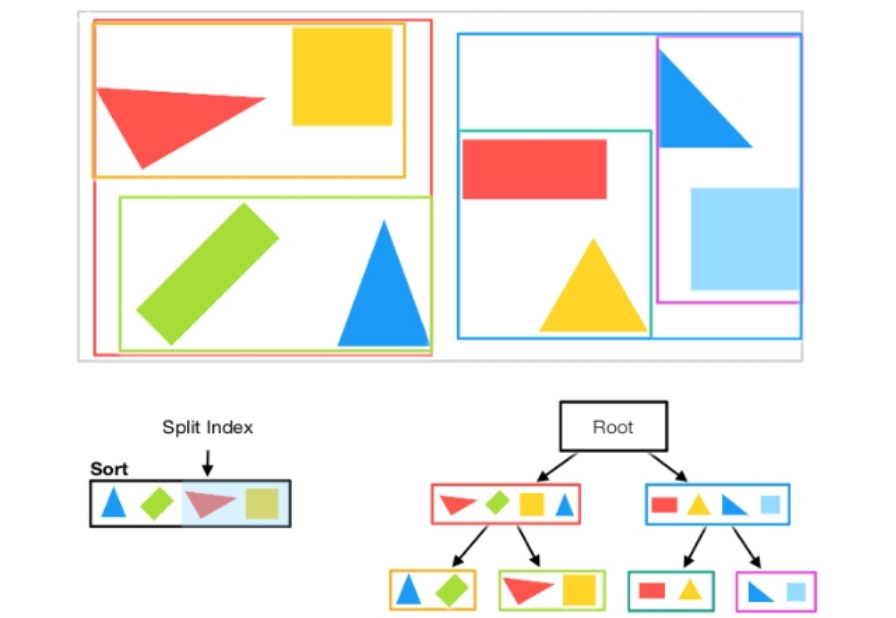
\includegraphics[width=6cm]{ImagesElio/BVH.png}
        \end{figure}
\end{tabular}

\end{frame}


%------------------------------------------------
\begin{frame}[fragile]
\frametitle{Parcours de BVH\esp}
\tiny 
\begin{algorithm}[H]
    \caption{\textsf{TraverseBVH}}
    \Input{Noeud racine $N=(S,l,g,d)$, position $p$}
    \Output{Plus courte distance de $p$ aux objets de la scène}
    \BlankLine
    Initialiser $d1$ à la distance entre $p$ et la sphère englobante gauche\;

    Initialiser $d2$ à la distance entre $p$ et la sphère englobante droite\;

    %{\footnotesize\tcc*{~La source est la racine de l’arborescence }}
    $dist \gets +\infty$\;
    %{\footnotesize\tcc*{~La racine est le premier sommet à traiter }}
    \If{$N$ est une feuille}{
        $dist \gets \min_i{(dist(p,l[i]))}$\;
    }
    \ElseIf{$d1 < d2$}{
        $dist \gets$ TraverseBVH($g, p$)\;
        \If{$d2 < dist$}{ 
            $dist \gets$ min($dist$, TraverseBVH($d,p$))\;
        }
    }	
    \Else{
        $dist \gets$ TraverseBVH($d, p$)\;
        \If{$d1 < dist$}{ 
            $dist \gets$ min($dist$, TraverseBVH($g,p$))\;
        }
    }
\Return{$dist$}
\end{algorithm}
\end{frame}


%------------------------------------------------
\begin{frame}[fragile]
\frametitle{Utilité et mise en pratique}

Implémentation en C de la structure d'objet :
\begin{lstlisting}[c]
Objet :
  Type    // cube, sphere...
  Centre          
  Rayon   // aide au calcul de sphere englobante
  Couleur
  Parametres  // sous forme de void*
\end{lstlisting}
\medskip

La structure de BVH :
\begin{itemize}
    \item est construite une seule fois pour des objets fixes.
    \item réduit les calculs pour une scène comportant beaucoup d'objets
\end{itemize}

\end{frame}


%++++++++++++++++++++++++++++++++++++++++++++++++
\subsection{Manipulation d'objets en mouvements}
%------------------------------------------------
\begin{frame}[fragile]
\frametitle{Gestion des objets en mouvement}
Construction de 2 arbres : 
\begin{itemize}
    \item Un BVH contenant les objets fixes calculé au début de la boucle
    \item Un BVH contenant les objets en mouvement recalculé pour chaque image
\end{itemize}
\\[1cm]

\end{frame}


%++++++++++++++++++++++++++++++++++++++++++++++++
\subsection{Bilan, gain de temps}
%------------------------------------------------
\begin{frame}[fragile]
\frametitle{Bilan et gains}
\label{derniere_slide_effective}
\end{frame}

Temps de génération et de libération de l'arbre négligeables (0,04s pour la scène 1)
\medskip 

\begin{tabular}{p{.5\textwidth}p{.5\textwidth}}
    \flushleft  
    Scène test 1 :  
    \medskip 
    
    \begin{figure}
        \includegraphics[width=5cm]{ImagesElio/Simpson.jpg}
    \end{figure}
    \medskip

    6500 triangles
    \smallskip

    6 threads, écran de 960x540 :

    \hspace{1cm}
    7min
    
        & \flushright 
        Scène test 2 : 
        \medskip 

            \begin{figure}[H]
                \includegraphics[width=5cm]{ImagesElio/Plage.jpg}
            \end{figure}
            \medskip 

            3000 triangles 
            \medskip 

            6 threads, écran de 960x540 :

            \hspace{1cm}
            40s
    \end{tabular}


%------------------------------------------------
\begin{frame}[fragile]
\frametitle{Slide bonus qui ne compte pas}
\end{frame}


%------------------------------------------------
\begin{frame}[fragile]
\frametitle{Encore une slide bonus qui ne compte pas}
\end{frame}
\addtocounter{framenumber}{-2} 





\end{document}
